\documentclass{beamer}

% \usepackage{beamerthemesplit} // Activate for custom appearance

\title{Math 493 Project 1}
\author{Aneesh \& JJ \& Matt}
\date{\today}

\begin{document}

\frame{\titlepage}

\section[Outline]{}

\section{Problem 1}
\frame
{
\frametitle{Problem 1}

\begin{align*}
x' &= \theta x^2 \\
x(1) &= -1
\end{align*}
}

\frame{
\frametitle{Sensitivity System 1}

\begin{itemize} 
\item We solved the following sensitivity system 
\begin{align*}
D
\begin{pmatrix} 
x \\ 
\partial_{\theta} x \\
\end{pmatrix} & = 
\begin{pmatrix} 
\theta x^2 \\
x^2 + 2\theta x (\partial_{\theta}x) \\
\end{pmatrix} \\ 
\begin{pmatrix} 
 x \\
\partial_{\theta}
\end{pmatrix}(1) &=
\begin{pmatrix}
-1 \\ 0
\end{pmatrix}
\end{align*}
\end{itemize} 
}

\frame{
\frametitle{Problem 1 Results}
\centering
\begin{tabular}{ccc}
Method & $\theta$ & SSE \\ \hline
fminsearch & 1.8432617 &  0.1313268 \\
Gauss-Newton & 1.8416666 & 0.1313271\\
\end{tabular}
}

\frame{
\frametitle{Problem 1 Results}
\begin{figure}
    \centering
    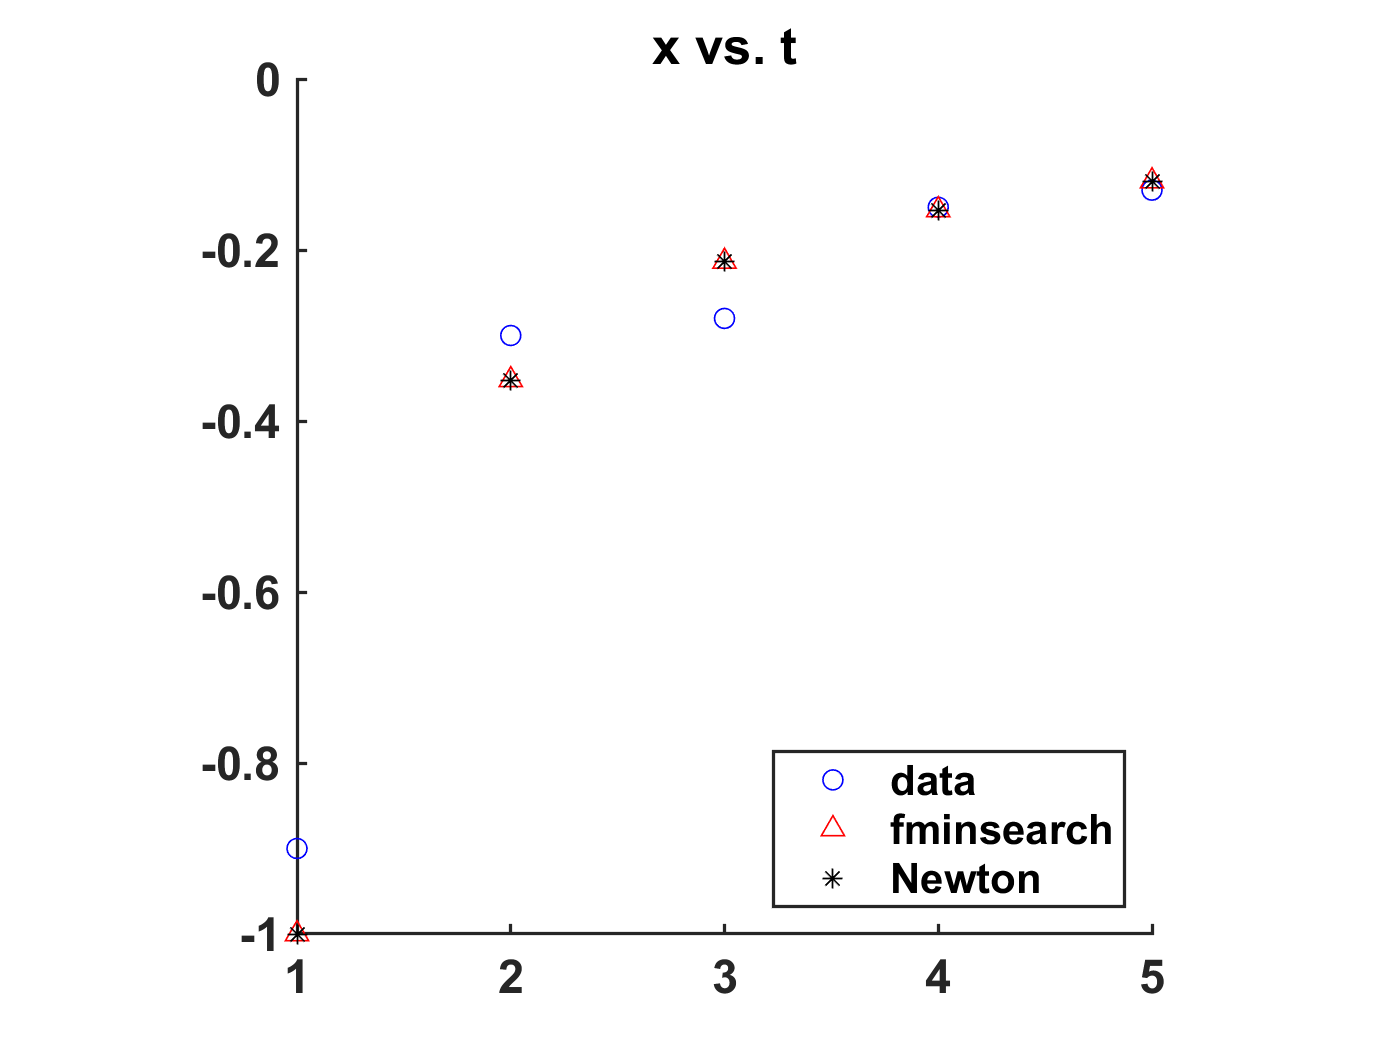
\includegraphics[scale=0.2]{Proj1_comparison.png}
    \caption{Approximations compared with data. It took fminsearch 16 steps while it took Gauss-Newton 12 steps to converge.}
\end{figure}

}

\frame{
\frametitle{Problem 1 Results}
\begin{figure}
    \centering
    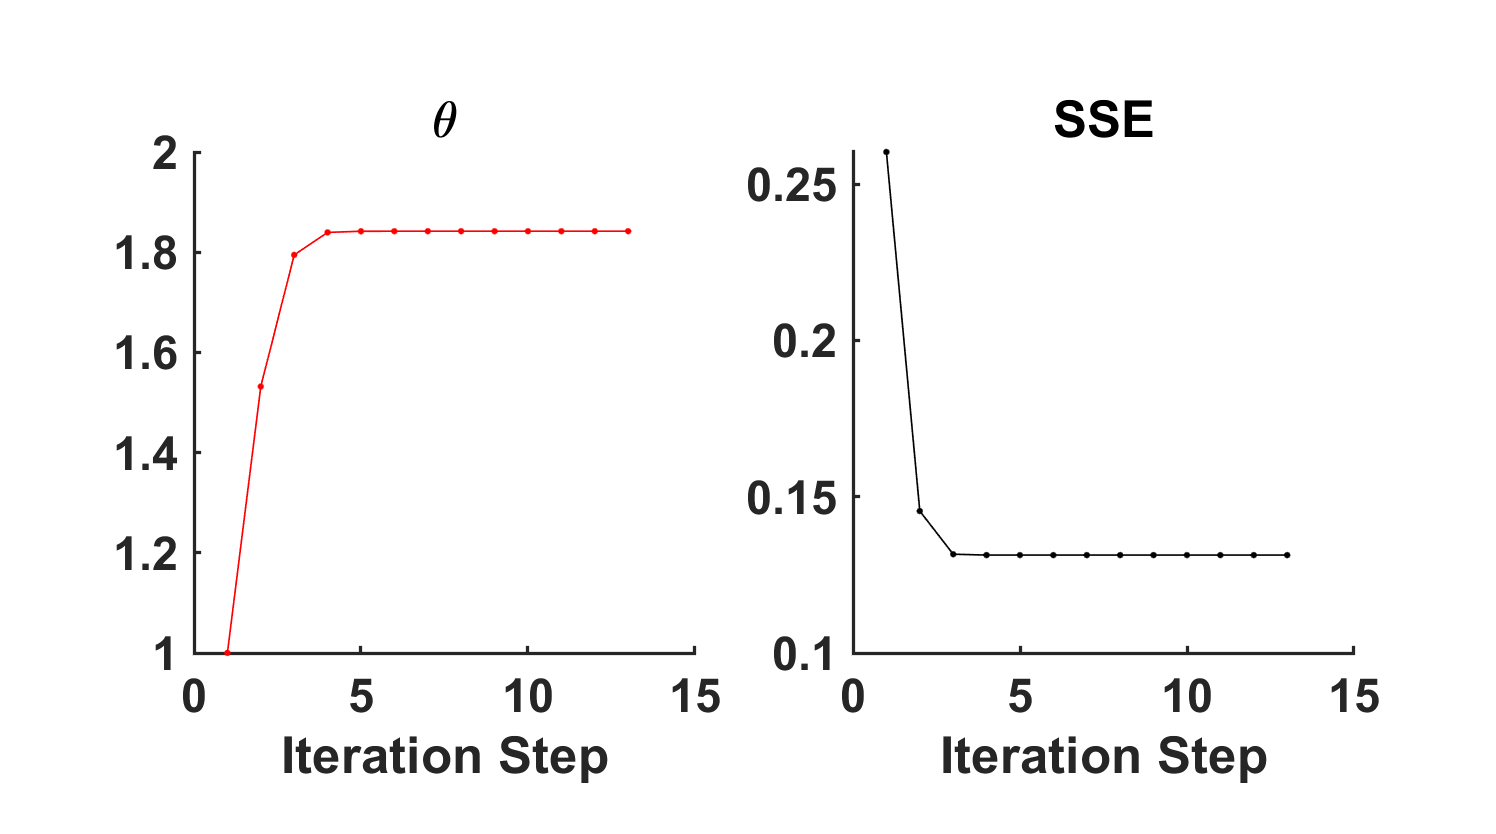
\includegraphics[scale=0.25]{Proj1_1_convergence.png}
    \caption{Convergence of Gauss-Newton}
\end{figure}
}


\frame{
\frametitle{Sensitivity System 2}
\begin{align*}
D
\begin{pmatrix}
    x \\
    \partial_\theta x \\
    \partial_{x_0} x \\
\end{pmatrix}
&=
\begin{pmatrix}
    x^2\theta \\
    x^2+2x\theta \partial_\theta x \\
    2x\theta \partial_{x_0} x
\end{pmatrix}
\end{align*}

\begin{align*}
\begin{pmatrix}
    x \\
    \partial_\theta x \\
    \partial_{x_0} x \\
\end{pmatrix}(1)
&=
\begin{pmatrix}
    -0.9 \\
    0 \\
    1\theta v
\end{pmatrix}
\end{align*}
}

\frame{
\frametitle{Problem 2 Results}
\centering
\begin{tabular}{cccc}
Method & $\theta$ & $x_0$ & SSE \\ \hline
fminsearch & 1.7553438 &  -0.8962938 &  0.0808069\\
Gauss-Newton & 1.7543119 & -0.8963022 & 0.0808071\\
\end{tabular}
}

\frame{
\frametitle{Problem 2 Results}
\begin{figure}
    \centering
    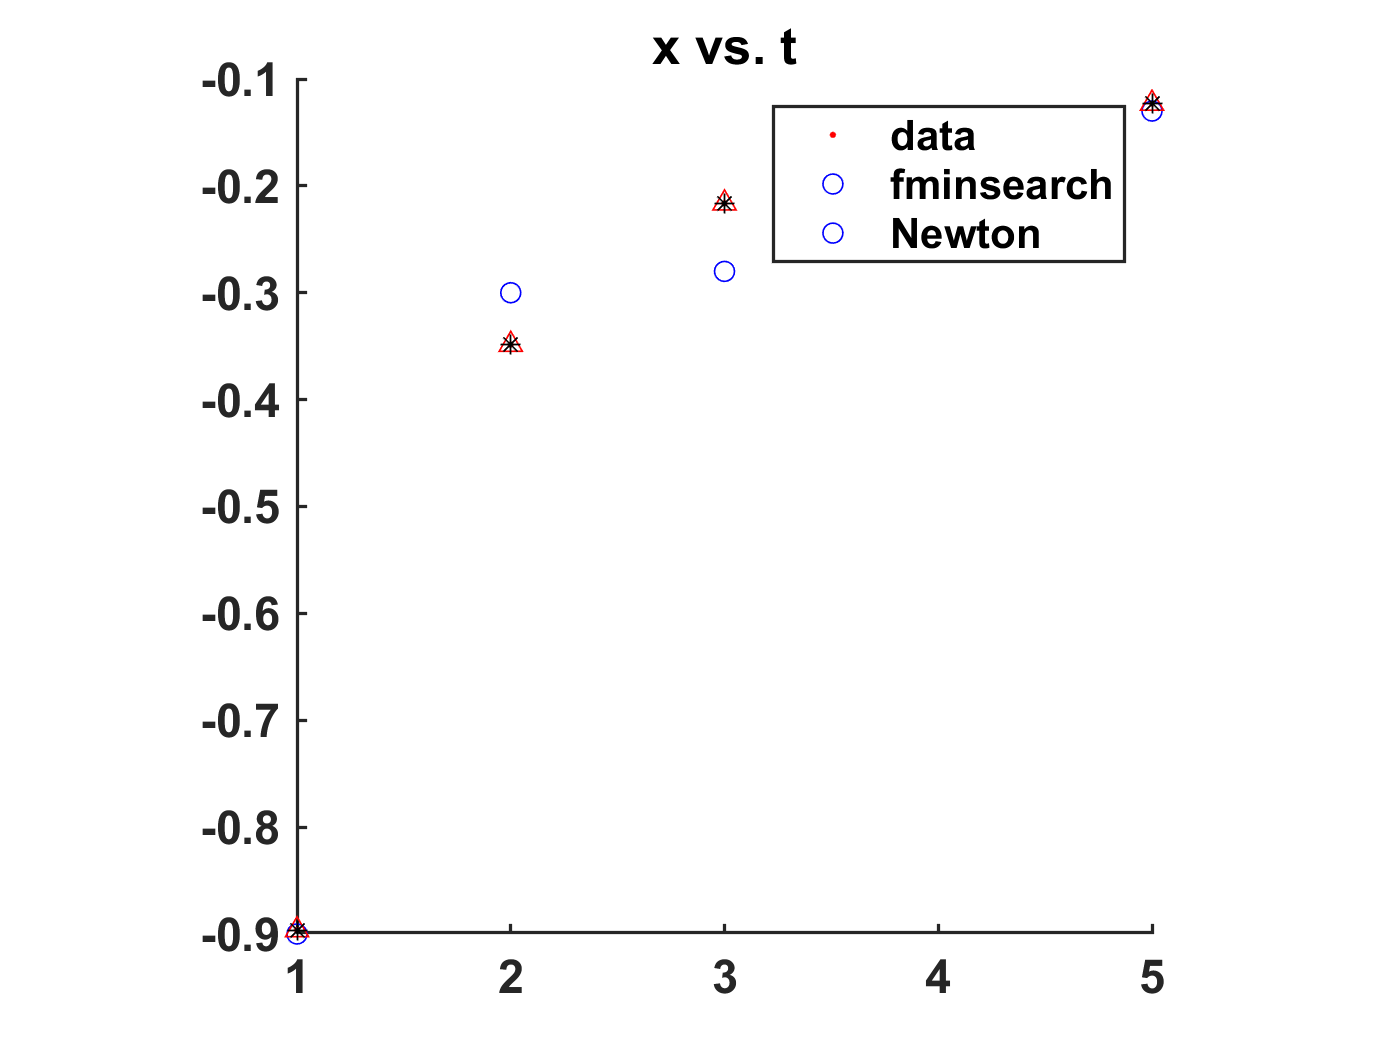
\includegraphics[scale=0.2]{Proj1_comparison2.png}
    \caption{Approximations compared with data. It took fminsearch 41 steps while it took Gauss-Newton 13 steps to converge.}
\end{figure}
}

\frame{
\frametitle{Problem 2 Results}
\begin{figure}
    \centering
    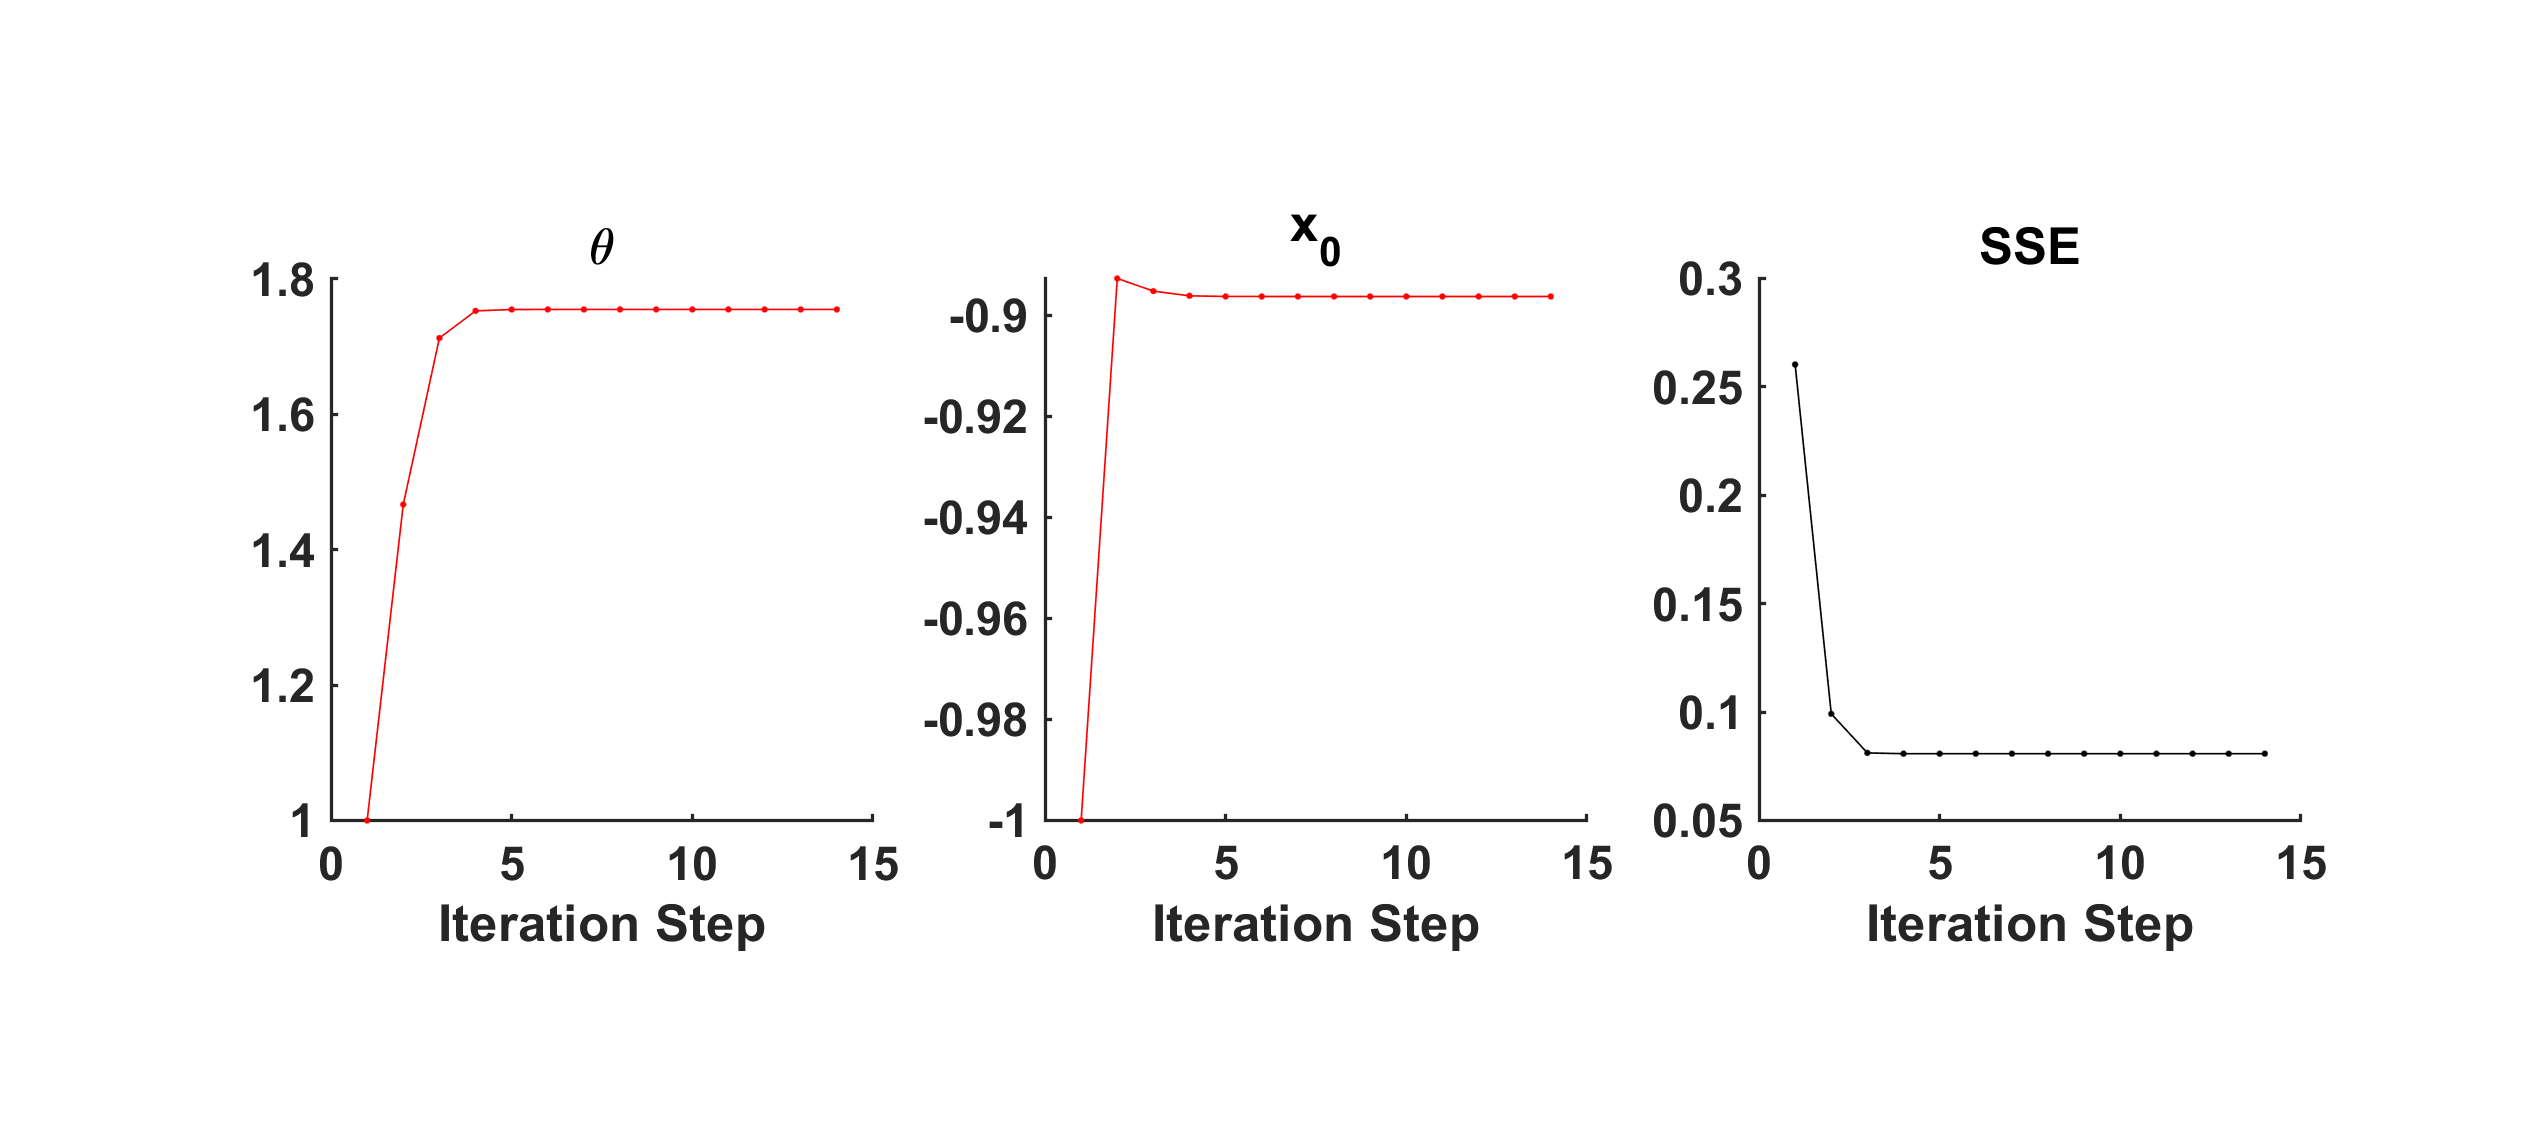
\includegraphics[scale=0.16]{Proj1_2_convergence.png}
    \caption{Convergence of Gauss-Newton}
\end{figure}
}



\frame{
\frametitle{Sensitivity System 3}
 \[D
\begin{pmatrix}
    x \\
    y \\
    \partial_a x \\
    \partial_a y \\
    \partial_b x \\
    \partial_b y
\end{pmatrix}
=
\begin{pmatrix}
    -axy \\
    axy-by \\
    -xy-ay\partial_ax-ayx\partial_ay \\
    xy+ay\partial_a x+(ax-b)\partial_ay \\
    -ay\partial_bx-ax\partial_by
    -y+ay\partial_bx+(ax-b)\partial_by
\end{pmatrix}
\]

 \[D
\begin{pmatrix}
    x \\
    y \\
    \partial_a x \\
    \partial_a y \\
    \partial_b x \\
    \partial_b y
\end{pmatrix}(0) =
\begin{pmatrix}
0.9\\
0.1\\
0 \\
0\\
1\\
1\\
\end{pmatrix}
\]
}

\frame{
\frametitle{Problem 3 Results}
\centering
\begin{tabular}{cccc}
Method & $a$ & $b$ & SSE \\ \hline
fminsearch & 0.5022775 &  0.1030516 &  0.0171071\\
Gauss-Newton & 0.5132331 &  0.1091130 & 0.0173460\\
\end{tabular}
}

\frame{
\frametitle{Problem 3 Results}
\begin{figure}
    \centering
    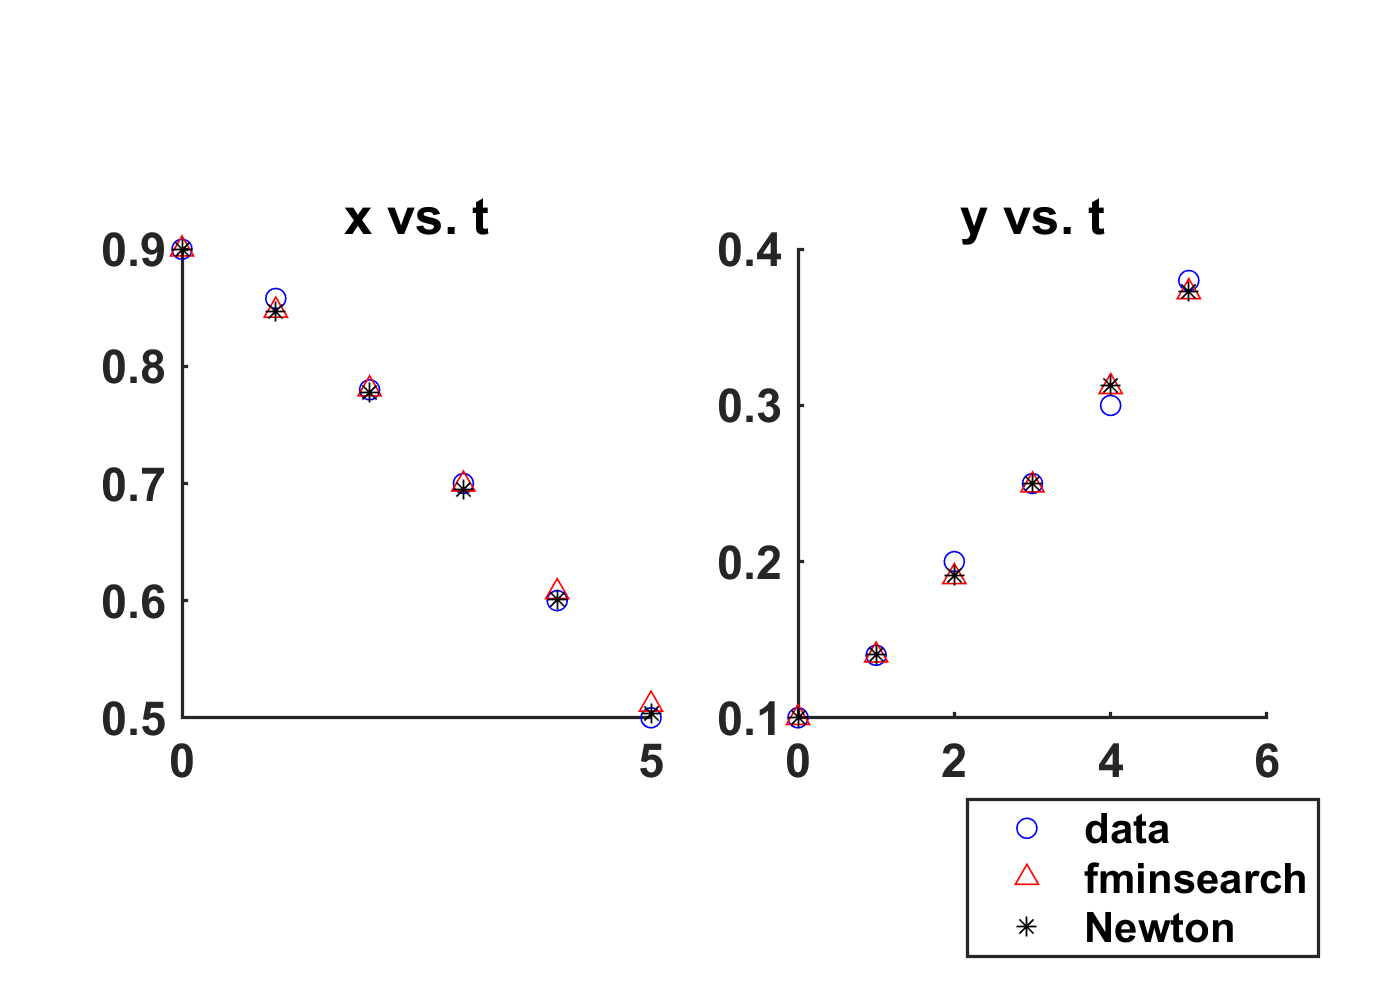
\includegraphics[scale=0.25]{Proj1_comparison3.png}
    \caption{Approximations compared with data. It took fminsearch 71 steps while it took Gauss-Newton 49 steps to converge.}
\end{figure}
}

\frame{
\frametitle{Problem 3 Results}
\begin{figure}
    \centering
    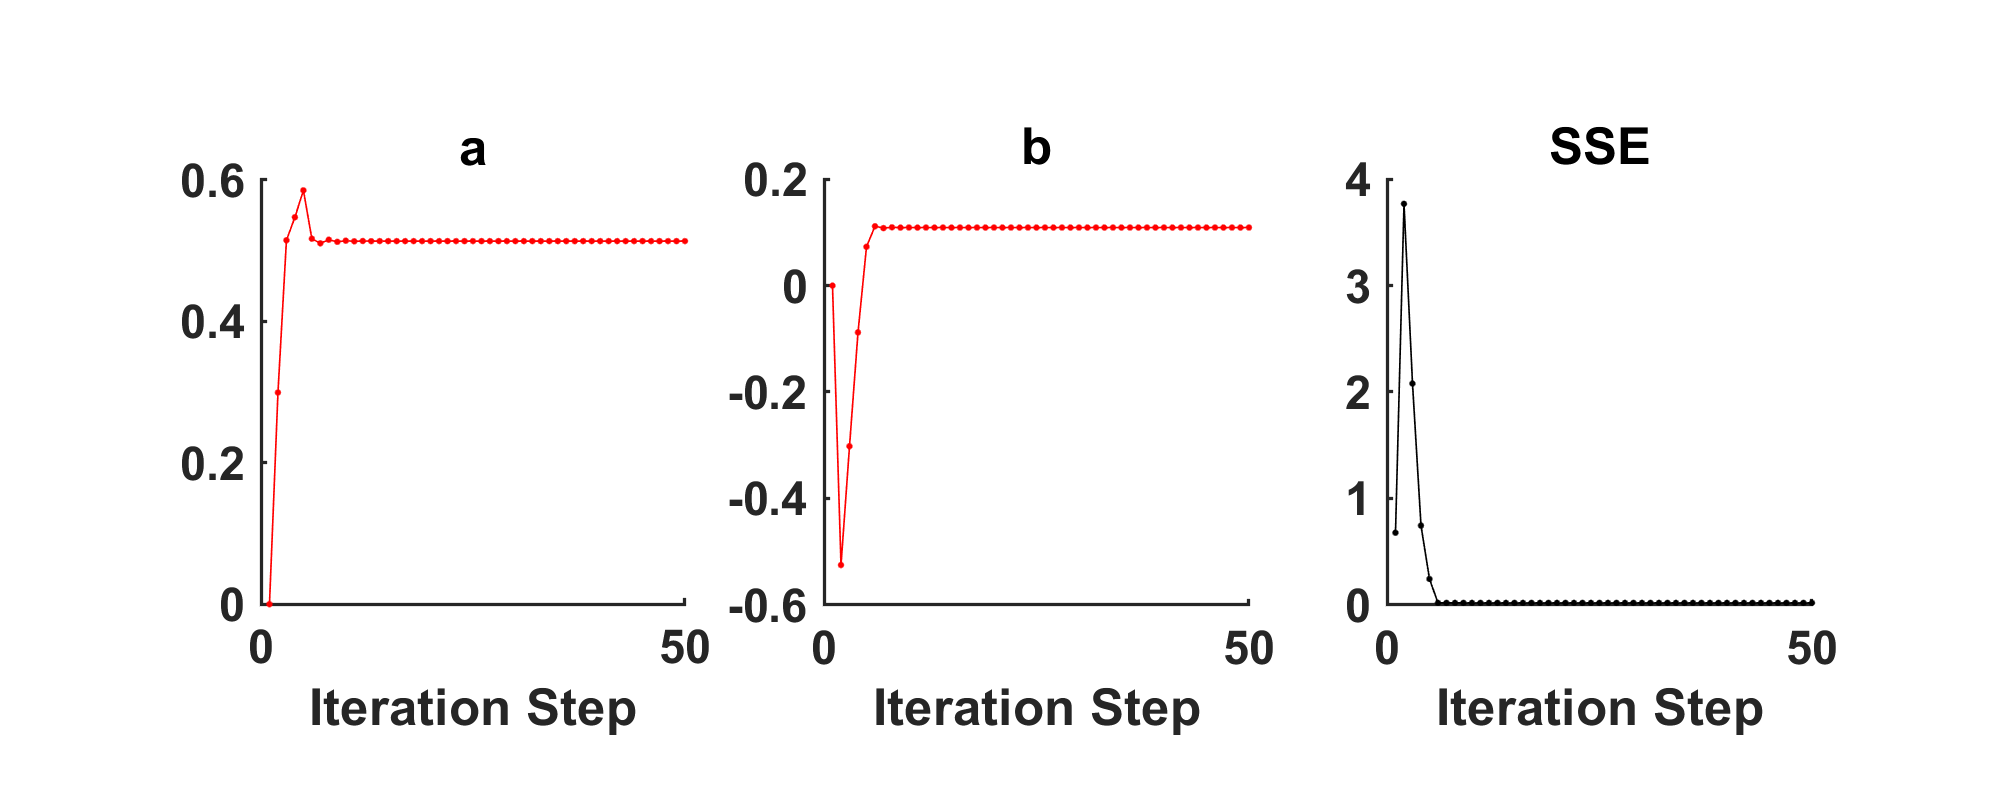
\includegraphics[scale=0.21]{Proj1_3_convergence.png}
    \caption{Convergence of Gauss-Newton}
\end{figure}
}

\frame{
\frametitle{Population Dynamic}
\begin{figure}
    \centering
    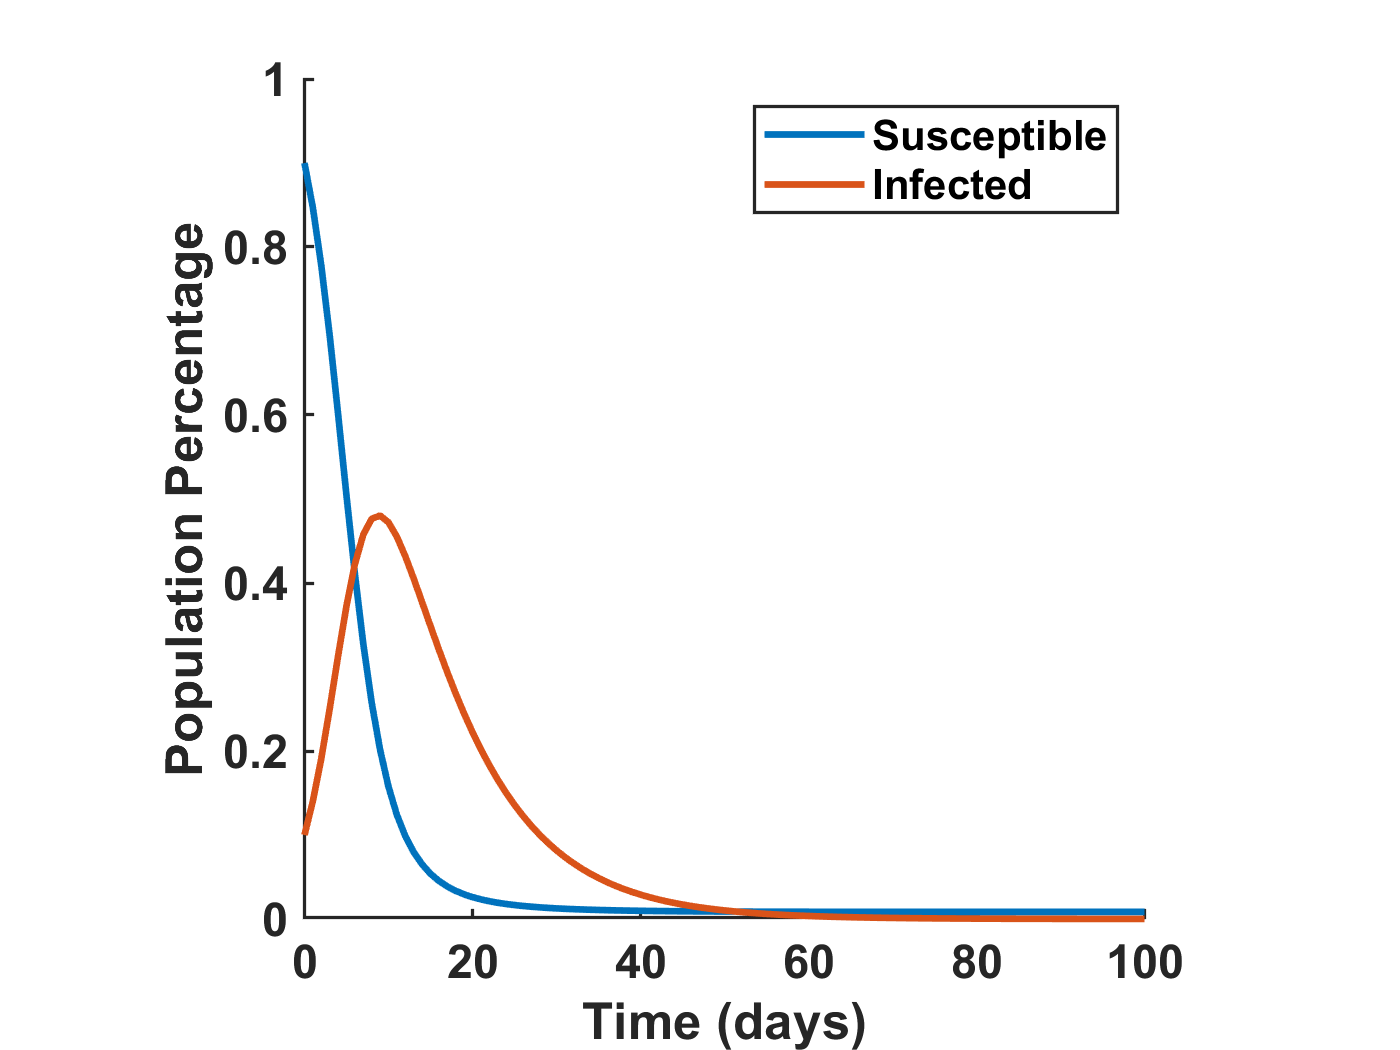
\includegraphics[scale=0.2]{Proj1_3_dynamic.png}
    \caption{Population percentage of susceptible and infected population}
\end{figure}
}

\end{document}
